% Auto-generated by gen_qual.py -- do not edit by hand.
% Needs in preamble: \usepackage{tikz}\usetikzlibrary{shadows,positioning,calc}
\definecolor{qRedFill}{RGB}{253,236,236}\definecolor{qRedLine}{RGB}{232,170,170}
\definecolor{qGrayFill}{RGB}{241,243,247}\definecolor{qGrayLine}{RGB}{190,197,210}
\definecolor{qGreenFill}{RGB}{236,247,236}\definecolor{qGreenLine}{RGB}{160,205,160}
\definecolor{qPromptFill}{RGB}{214,214,214}\definecolor{qHal}{RGB}{204,0,0}\definecolor{qHalBg}{RGB}{255,170,170}
\providecommand{\halobj}[1]{{\setlength{\fboxsep}{0.4pt}\colorbox{qHalBg}{\textcolor{qHal}{\textbf{#1}}}}}
\begin{tikzpicture}[font=\sffamily\fontsize{6.9}{8.3}\selectfont,box/.style={rounded corners=3pt, draw, line width=0.5pt, inner sep=3.2pt, align=justify,text width=4.405in, drop shadow={opacity=0.18, shadow xshift=0.6pt, shadow yshift=-0.8pt}}]
\node[box, fill=qPromptFill, draw=qPromptFill, anchor=north west] (p480140) at (2.340in,0.000in) {\textbf{Prompt:} Please describe this image in detail.};
\node[box, fill=qRedFill, draw=qRedLine, below=2.6pt of p480140.south west, anchor=north west] (r4801400) {\textbf{Regular:} The image depicts a busy city street with a group of people walking across the street at a crosswalk. There are at least nine people visible in the scene, some of them carrying handbags. A man is walking with a \halobj{frisbee} in his hand, adding a playful element to the scene. The street is filled with various vehicles, including cars and a bus. There are at least six cars and one bus in the image, with some of them parked or stopped at the crosswalk. The presence of multiple traffic lights indicates that the area is well-regulated for pedestrian and vehicular safety.};
\node[box, fill=qGrayFill, draw=qGrayLine, below=2.6pt of r4801400.south west, anchor=north west] (r4801401) {\textbf{Static gate:} The image depicts a busy downtown area with many people crossing the street. Pedestrians are seen crossing at crosswalks, while drivers are patiently waiting for them. Several cars are parked or driving down the street, and some are stopped at red lights. Pedestrians are carrying handbags, and some are wearing \halobj{backpacks}. Traffic lights can be seen at different points, controlling the flow of vehicles. Buildings line the street, contributing to the downtown feel.};
\node[box, fill=qGreenFill, draw=qGreenLine, below=2.6pt of r4801401.south west, anchor=north west] (r4801402) {\textbf{EGDR (ours):} The image depicts a busy downtown area with many people crossing the intersection. Pedestrians are seen crossing the crosswalk, while drivers are patiently waiting for them. Several cars are parked or driving through the intersection, with some visible in the foreground, middle, and background. Pedestrians can be seen carrying handbags, with at least three visible. Traffic lights are installed at the intersection, controlling the flow of vehicles. One of them is red, signaling for drivers to stop.};
\path let \p1=(p480140.north), \p2=(r4801402.south) in node[rounded corners=4pt, fill=qGrayFill, draw=qGrayLine, line width=0.5pt, minimum width=2.180in, minimum height=\y1-\y2, anchor=north west, drop shadow={opacity=0.18, shadow xshift=0.6pt, shadow yshift=-0.8pt}] (f480140) at (0,\y1) {};
\begin{scope}\clip[rounded corners=3pt] ($(f480140.center)+(-1.050in,-0.913in)$) rectangle ++(2.100in,1.826in);\node[inner sep=0pt] at (f480140.center) {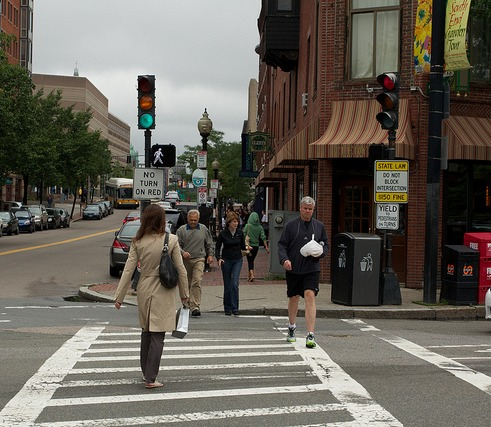
\includegraphics[width=2.100in]{qual_480140.jpg}};\end{scope}
\node[anchor=south, inner sep=0pt, text=black!55, font=\sffamily\fontsize{5.6}{6.5}\selectfont] at ($(f480140.south)+(0,0.05in)$) {COCO val2014 \textperiodcentered\ ID 480140};
\end{tikzpicture}
